\documentclass{article}
\usepackage[utf8]{inputenc} %кодировка
\usepackage[T2A]{fontenc}
\usepackage[english,russian]{babel} %русификатор 
\usepackage{mathtools} %библиотека матеши
\usepackage[left=1cm,right=1cm,top=2cm,bottom=2cm,bindingoffset=0cm]{geometry} %изменение отступов на листе
\usepackage{amsmath}
\usepackage{graphicx} %библиотека для графики и картинок
\graphicspath{}
\DeclareGraphicsExtensions{.pdf,.png,.jpg}
\usepackage{subcaption}
\usepackage{pgfplots}
\usepackage{amssymb}

\begin{document}
% НАЧАЛО ТИТУЛЬНОГО ЛИСТА
\begin{center}
    \Large
    Федеральное государственное автономное \\
    образовательное учреждение высшего образования \\ 
    «Научно-образовательная корпорация ИТМО»\\
    \vspace{0.5cm}
    \large
    Факультет программной инженерии и компьютерной техники \\
    Направление подготовки 09.03.04 Программная инженерия \\
    \vspace{1cm}
    \Large
    \textbf{Отчёт по лабораторной работе №3} \\
    По дисциплине «Базы данных» (второй семестр)\\
    \large
    \vspace{8cm}

    \begin{minipage}{.33\textwidth}
    \end{minipage}
    \hfill
    \begin{minipage}{.4\textwidth}
    
        \textbf{Студент}: \vspace{.1cm} \\
        \ Дениченко Александр P3112\\
        \textbf{Практик}:  \\
        \ Лисицина В.В
    \end{minipage}
    \vfill
Санкт-Петербург\\ 2023 г.
\end{center}

% КОНЕЦ ТИТУЛЬНОГО ЛИСТА 
\newpage

\section{ФНП и скалярное поле}
П.1 Основные понятия\\


$\mathbb{R} x \mathbb{R} x \mathbb{R} ... x \mathbb{R} = \mathbb{R}^n = \{(x_1, x_2, .., x_n): x_i \in \mathbb{R}, i = 1 ... n\}\\
\mathbb{D} \in \mathbb{R}^n \\
n = 2 (x,y)$


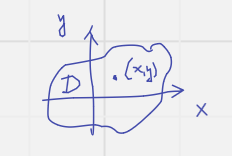
\includegraphics[width=.3\textwidth]{1.1} 



Ограниченность $\mathbb{D} $ - ограничена, если существует  M>0 Для любых $(x, y) \in \mathbb{D} \sqrt{x^2+y^2}\in \leq \delta(M, O) \leq M$

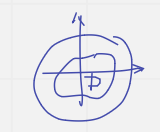
\includegraphics[width=.3\textwidth]{1.2} 

Внутренняя точка (IntD) M(x, y) - внутренняя, если существует $\mathcal{E} > 0 : U_{\mathcal{E}}(M) \in D $ == $\{(x', y'): \sqrt{(x-x')^2+(y-y')} < \mathcal{E}\}$

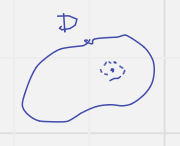
\includegraphics[width=.3\textwidth]{1.3} 

Граничная точка (знак частных производных)$\mathcal{D}$): M(x, y)
- граничная точка, если существует $\mathcal{E} > 0 : U^{\cdot}_{\mathcal{E}}(M) \cap \mathcal{D} != \bar{0}\  and\  U^{\cdot}_{\mathcal{E}}(M) \cap \bar{\mathcal{D}} != \bar{0}$


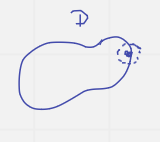
\includegraphics[width=.3\textwidth]{gran} 


Изолированная точка: существует $\mathcal{E} > 0 : U^{\cdot}_{\mathcal{E}}(M) \cap \mathcal{D} = \bar{0}$

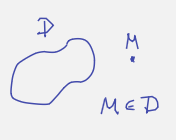
\includegraphics[width=.3\textwidth]{isolate} 


$\mathcal{F}: \mathcal{D} -> \mathbb{R}\ \forall(x, y) \in \mathcal{D}\ and \ \forall(x, y)\in \mathcal{D}\ =>\ !z \in \mathbb{R}: z = f(x,y)$

$\mathcal{D}$ - облать определения

E -множество точек

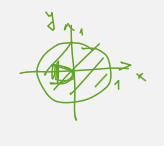
\includegraphics[width=.3\textwidth]{ddd} 
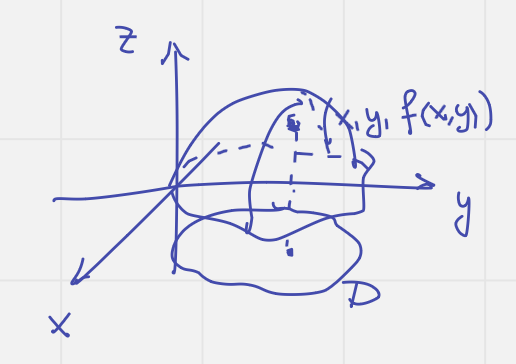
\includegraphics[width=.3\textwidth]{2} 


Г $= \{(x, y, f(x,y)): (x, y) \in \mathcal{D}\}$ -график 

Пример: 
$z = \sqrt{1-x^2-y^2}$

$\mathcal{D} = \{(x, y): x^2 + y ^2 \leq 1\}$

\begin{equation}
    \begin{cases}
        x^2+y^2+z^2 = 1\\
        z \geq 0
    \end{cases}
\end{equation}

E = [0; 1]

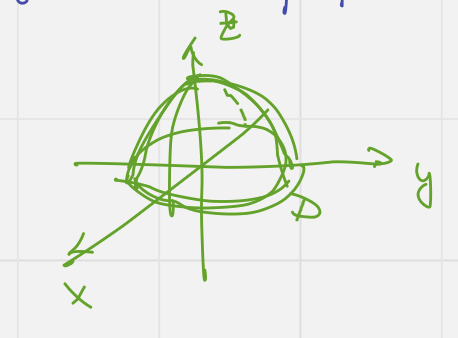
\includegraphics[width=.3\textwidth]{3} 
\\ \\
П.2 Линии и поверхности уровня

n = 2 $f: \mathcal{D} -> \mathbb{R}$

$L_c = \{(x, y): f(x, y = c )\}$

$S_c = \{(x, y, z): f(x, y, z = c )\}$

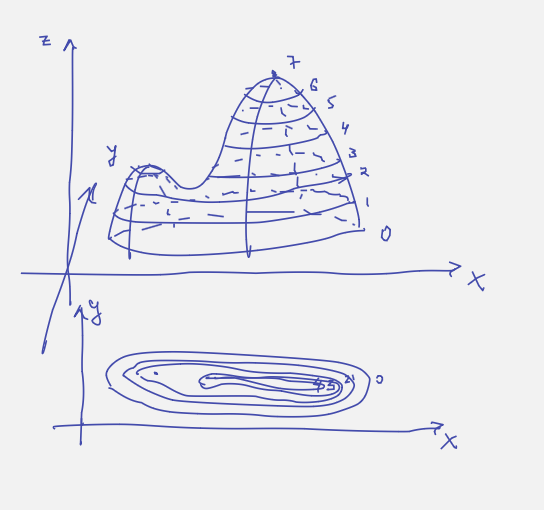
\includegraphics[width=.3\textwidth]{line} 
\\ \\
п.3 Частное и полное приращение 

$f: \mathcal{D} -> \mathbb{R}$, n=2

z = f(x, y)

$\Delta z = f(x+ \Delta x, y + \Delta y) - f(x, y)$

полное приращение

$\Delta_x z = f(x+ \Delta x, y) - f(x, y)$

частное приращение по переменной x

$\Delta_y z = f(x, y + \Delta y) - f(x, y)$

частное приращение по переменной y

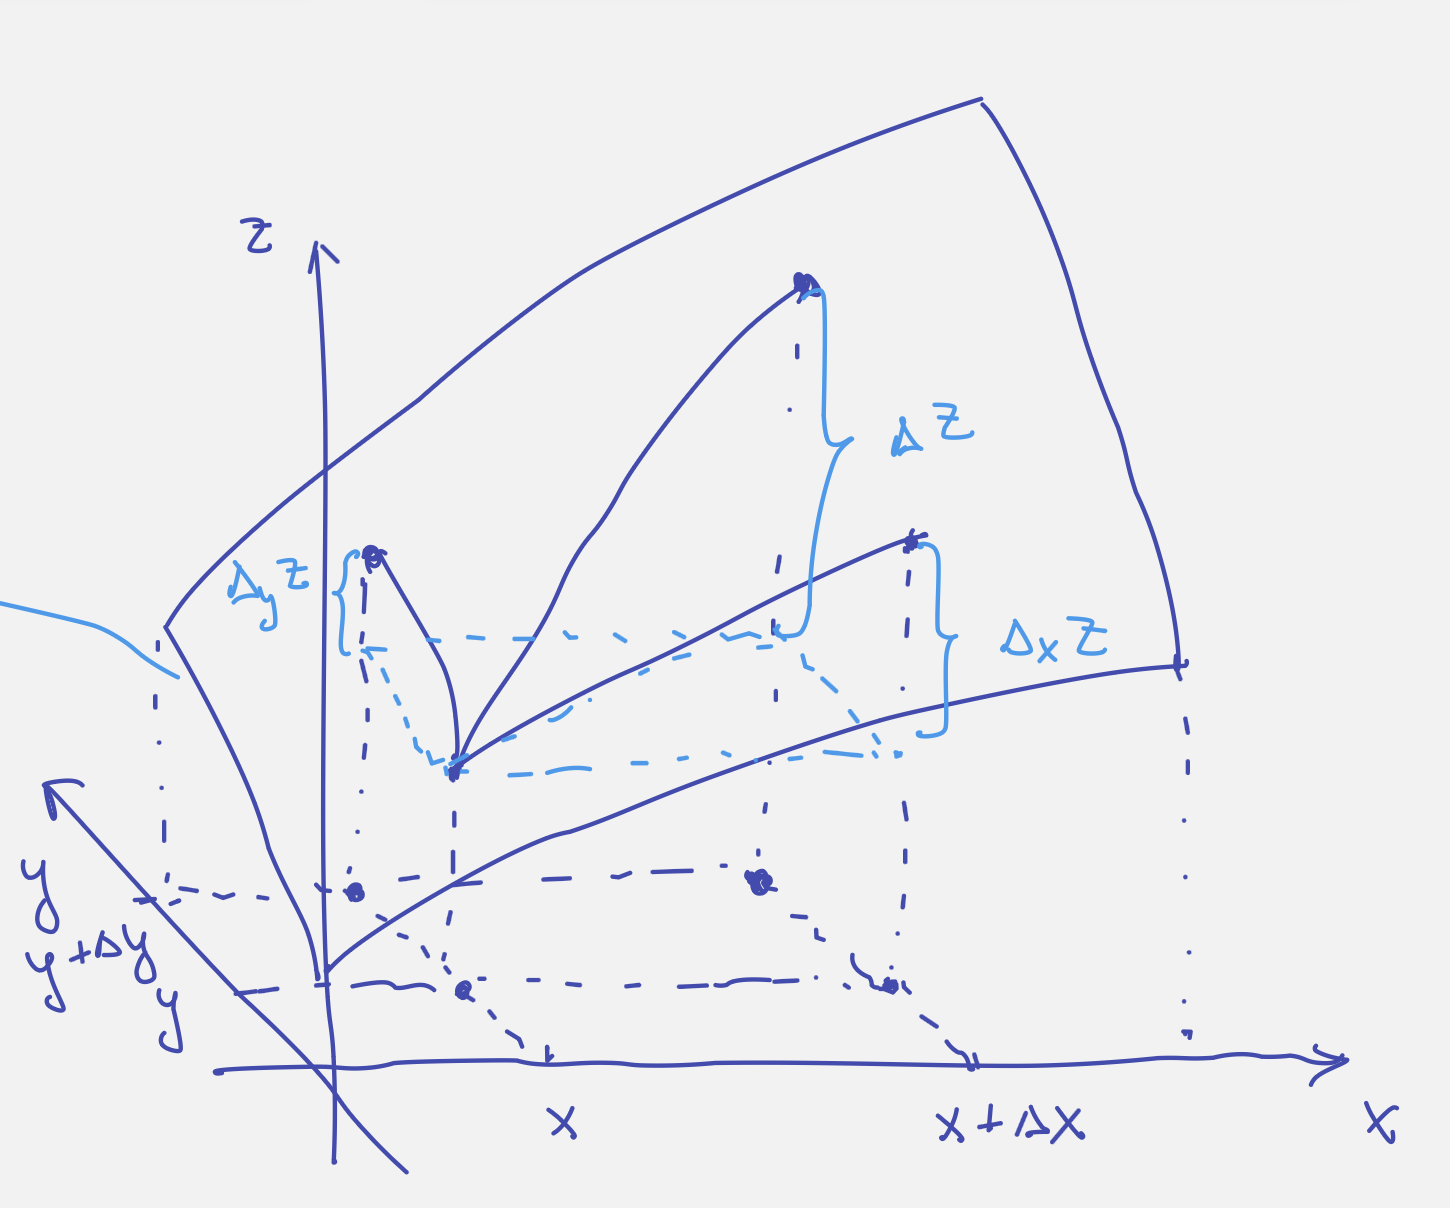
\includegraphics[width=.4\textwidth]{prir.png} 

$\Delta z != \Delta_x z + \Delta_y z $

Пример: 

S = xy

x=1 $\Delta x =0,1 $

y=2 $\Delta y =0,2 $

$\Delta S = (x+\Delta x)(y+\Delta y) - xy = x \Delta y + y \Delta x +\Delta x \Delta y = 0,42$


$\Delta_x S + \Delta_y S = (x + \Delta x)y - xy + (y +\Delta y)x  - xy = \Delta x \cdot y + \Delta y \cdot x$


п.4 Предел и непрерывность 

$\lim_{x -> x_0}f(x) = A\ <=>\ \forall \mathcal{E} >0 \ \exists \delta_{\mathcal{E}}>0 : \forall x \in U^{\cdot}_{\delta}(x_0) \cap \mathcal{D}_f => f(x) \in U_{\mathcal{E}}(A)$


$\lim_{M -> M_0}f(M) = A\ <=>\ \forall \mathcal{E} >0 \ \exists \delta_{\mathcal{E}}>0 : \forall M \in U^{\cdot}_{\delta}(M_0) \cap \mathcal{D}_f => f(M) \in U_{\mathcal{E}}(A)$
\\ \\
$M(x, y), M(x_1, y_1)$
\\ \\
1) $z = x^2 +y^2 \mathcal{D} = \mathbb{R}^2 \Delta z= (x_0 + \Delta x)^2 + (y+ \Delta y)^2 - x_0^2 - y_0^2 = 2x_0 \Delta x + \Delta x^2 +2y_0\Delta y + \Delta y^2 - (\Delta x ->0,  \Delta y ->0) -> 0 $

z - непрерывная на $\mathcal{D} = \mathbb{R}^2$

$\lim_{(x, y)-> 0)}(\frac{2xy}{x^2 +y^2}) = |y = kx| = \lim_{(x, y)-> 0)}(\frac{2xkx}{x^2 +(kx)^2}) = \frac{2k}{1+k^2} предел не существует
$

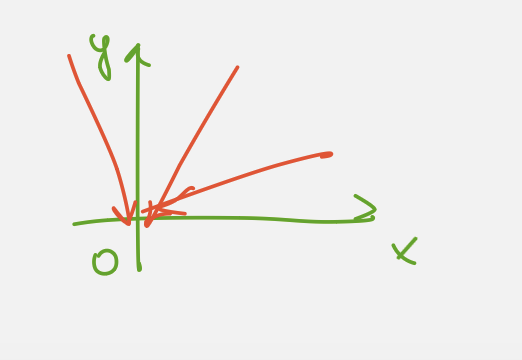
\includegraphics[width=.3\textwidth]{lines} 
\end{document}
